\documentclass[11pt, rgb]{scrreprt}
\usepackage{themeKonstanzDBIS} % Muss immer verwendet werden (Standardpaket)

\usepackage{algorithm}
\usepackage{algorithmicx}
\usepackage{algpseudocode}
\usepackage{mathtools}  % amsmath with extensions
\usepackage{amsmath} 
\usepackage{amsfonts}  % (otherwise \mathbb does nothing)
\usepackage{amssymb}  % (otherwise \mathbb does nothing)
\usepackage{nameref}


\format{a4}

% Thesis information        %
%\date{\today}
\year{2023}
\author{Marius Hahn}
\title{MSc Thesis}
\subtitle{thesis}
\unisection{Faculty of Sciences}
\department{Department of Computer and Information Science}
\supervisorOne{Prof. Dr. Theodoros Chondrogiannis}
\supervisorTwo{Prof. Dr. Sabine Storandt}

\headFoot{14}

%%%%%%%%%%%%%%%%%%%%%%%%%%%%%%%%%%%%%%%%%%%%%%%%%%%%%%%%%
% Begin vom Dokument                                    %
%%%%%%%%%%%%%%%%%%%%%%%%%%%%%%%%%%%%%%%%%%%%%%%%%%%%%%%%%

\begin{document}

% Thesis Title
\thesistitlepage[language=english]{MSc Thesis Title}

\chapter*{Abstract}

% Table of Contents           
\tableofcontents

%Use only if thesis is over 100 pages.
% List of figures
%\listoffigures
%\addcontentsline{toc}{chapter}{List of Figures}

%Use only if thesis is over 100 pages.
% List of tables
%\listoftables
%\addcontentsline{toc}{chapter}{List of Tables}

% For chapters and sections use  
%    \chapter{...}
%    \section{...}
%    \subsection{...}
%    \subsubsection{...}
%

\rmfamily 
\normalsize

\chapter{Introduction}

Most applications which handle data have to store these eventually.
Simple files do not offer enough semantic structure.
Therefore databases have been developed to not only store but query and aggregate data effectively and efficiently.
Relational databases that store data in tables have become the unspoken industry standard in the last decades. 
However there are domains that do not naturally fit into tables and one will need a lot of restructuring to make them fit.
As a result, there have been efforts to create databases that use other abstractions to store data, like the graph database Neo4j.

\section{Background and Motivation}

In a relational database the data is organized in tables.
Tables have rows and theses rows can be connected to other rows of the same or a different table using joins on matching cells, usually primary- foreign key relationships.
To retrieve information that is stored in two table rows one has to scan both an join them on the desired key property.
Depending on the size of the tables and the number of joins which have to be done to retrieve the desired information, such queries can be very expensive.
\\
In contrast to relational databases, graph databases treat relationships as first-class citizen.
This means a relationship that connects nodes is an entity just as the nodes it connects themselves.
As in a graph database, a node has a pointer to its relationship and a relationship has a pointer to its nodes, there is no table scan needed to retrieve connected data, which can make these queries very performant.
Such queries are shortest path queries on domains which resembles a graph by their nature, for instance road networks. 

\section{Problem and Objectives}

We focus on these shortest path queries and try to make these even quicker by employing an index call Customization Contraction Hierarchies \cite{CCH}, \textit{CCH}. 
CCH is proven to achieve a tremendous speedup compared to Dijkstra's algorithm in graphs where one can find vertices that are more important than others.
Important in this context means that these vertices belong to many shortest paths.
One example for such a domain are road networks, which we will also use in our test scenarios.

\section{Contribution}

In comparison to many other papers that examine CCH in their specific details we want to examine if we can adopt it to the graph database Neo4j, and still keep its advantages.
Will we be able to store the index in a manner which allows us to keep the performance gain we had achieved before?
Additionally we want to explore how the index behaves after updating multiple edge weights.
Will queries still be as quick as they were before the update?
This is an essential question as data in databases are usually not only stored but also manipulated.
We also want to uncover how big such an index graph will become, as there might be no need to read the index from the disk, because it easily fits in main memory.
\\
Finally we want to keep the integration into Neo4j as small as possible to make it as easy as possible at a later point to port the implementation to other graph databases that might become more relevant in future.

\chapter{Related Work} 

As this is mainly a database paper, we want to divide this chapter in two main sections \nameref{sec:algorithmic_history} and \nameref{sec:related_work:database}. \nameref{sec:algorithmic_history} 
that will give some basic overview what has been published regarding index structures to speed up shortest path queries for graphs. \nameref{sec:related_work:database} we will try 
to give an overview of efforts that have been made to make \cite[Customizable Contraction Hierarchies]{CCH} it suitable for graph databases.

\section[Algorithmic History]{Algorithmic History} \label{sec:algorithmic_history}

\cite[Contraction Hierarchies]{Geisberger_2012} or CH is heavily influenced by the idea of the \cite[Transit-Node]{Bast_2007} approach and as transit node approach itself, CCH is a
technique to speed up \cite[Dijkstras Algorithm]{Dijkstra_1959}, which is the most basic and robust algorithm to find shortest path in graphs. CH goes back to the diploma thesis of \cite[Geisberger]{Geisberger} in 2008. The \cite[Transit-Node]{Bast_2007} approach
tries to find vertices inside the graph that are more important than others. Important in this case means, these are vertices that reside on many shortest paths. This speeds up 
especially long distance queries, as one only needs to calculate the distance to the the next transit node of the source and target vertex as the shortest paths between 
the transit or access nodes will be known. \\ 
CH goes even further on the idea of having important vertices. It applies an importance to each vertex in the graph a so called rank. Furthermore it adds edges to the graph,
so called shortcuts, that preserve the shortest path property of the graph in case a vertex that is contracted resides on a shortest path between others. When querying a shortest
path CH uses a modified bidirectional-dijkstra that is restricted to only visit nodes that are of higher importance, or rank, than the its about to expand next.
This method is able to retrieve shortest paths of vertices that have a high spacial distance, however, it is rather static. In case a new edge is added or an edge weight is updated, 
it might be necessary to recontract the whole graph to preserve the shortest path property. \\
In 2016 \cite[Customization Contraction Hierarchies]{CCH} or CCH was published. The approach is the same, but in CCH shortcuts are not only added if the contraction violates the shortest path property,
they are added if there had been a connection between its neighbors through the just contracted vertex and these neighbors do not own a direct connection through an already existing edge.
The shortcut weights are later on calculated through the lowers triangle. Additionally the \cite[Customization Contraction Hierarchies]{CCH} provides an update approach that only updates,
edges that are affected by a weight change.

\section{Contraction Hierarchies Database History}\label{sec:related_work:database}

There is one bachelor thesis by Nicolai D'Effremo \cite[Some text]{DEffremo2019} that has implemented a version on \cite[Contraction Hierarchies]{Geisberger_2012} for Neo4j, one 
of the most used graph databases of today in 2023. This implementation shows that even in for databases CH is an index structure worth pursuing, as there was a tremendous speedup 
of shortest path queries paired with a reasonable preprocessing time. \cite{Zickenberg2021} showed in his bachelor thesis that it is even possible to restricted these
queries with label constraints. Although CH and CCH have little difference, sadly we could not use much of the code provided by there works. It
was deeply integrated into the Neo4j-Platform and since then two major release updates happened that have breaking changes which make it nearly impossible to reuse any of
this code.\\

Finally there is \cite[Mobile Route Planning]{Sanders} by Peter Sanders, Dominik Schultes, and Christian Vetter. In this paper it is described how one can efficiently store
the a CH index structure on a hard drive. It states an interesting technique to how store edge that are likely to be read sequentially spatially close on the hard drive which 
makes read operations that have to be done during query time fast. The motivation of \cite[Mobile Route Planning]{Sanders} through was slightly different. They came up with this
idea because computation power on mobile devices is limited, so they could precalculate the CH index on a server and then later distribute it to a mobile device.
\\
We will use parts of this idea and partly port it to our database context as we suppose there are many similarities.

\chapter{Preliminary}

As the target platform for this work is the graph database neo4J, we will mostly consider \textit{directed} graphs. From the terminology we always refer \textit{arcs}, which is an directed edge.
In some rare cases we might refer to \textit{edges}. There you can be sure that it doesn't matter weather it is directed or not.

\section{Notation and Expressions}
We denote a graph $G(V, A)$ in case me mean an \textit{directed} graph, where $v$ is a vertex contained in the vertices $v \epsilon  V$ and $e$ is an
edge $a \epsilon A$. An arc is uniquely defined by to vertices $v_a$ and $v_b$ such that $v_a \neq v_b$, so there are no loops nor multi edges.
An edge additionally has a weight function $w: E \rightarrow \mathbb{R}_{<0} $ it's weight which must be a positive.
\\
$G$ represents the input graph. The contraction graph $G'(V', A')$ is the graph that will be used at contraction for initially building the CCH index structure. A vertex $v$ in will 
never be really deleted. Instead the rank property $r(v)$ is set to mark this as an already contracted. So $V \equiv V'$ but $A \subseteq A'$ there will be edges add while building
the CCH index. $S = A' \setminus A$ is the shortcut set that is added throughout the contraction. 
\\
$G^*(V^*, A^*)$ is the is the search graph while doing one a shortest path query. Futhermore one query will have two search graphs. $G^*_\uparrow$ representing the upwards search graph
and the $G^*_\downarrow$.
\\
Finally there will be the edge set of edges that are written to the disk. These will $\bigcirc E$ will be separated into to sets $\bigcirc E_\downarrow$ and $\bigcirc E_\uparrow $, too.


\section{Customizable Contraction Hierarchies}\label{sec:Preliminary_CCH}


\chapter{Integration in a Neo4j}

In this section it is described how "Customizable Contraction Hierarchies" CCH is integrated into Neo4j. CCH arguments the input graph, which means it inserts arcs, so called shortcuts, that do not belong to the original data. To keep the change to the input graphs as little as possible we decided to not insert any arc into the graph that is stored inside the neo4j database, but introduce another graph data structure, the index graph. This index graph has an mapping to the input graph that is held by the database, by inserting two properties into the node of the input graph. The \textit{rank} this vertex has in the index graph and the \textit{indexing weight} it had during the last customization process. This gives yet another two advantages. One is that we get full control about the graph representation which is helpful to efficiently store and read the index graph for the disk. Another is that the with this approach it makes it easier to later on port the idea to another graph database manufactures.

\section{Index Graph Data Structure}\label{sec:index_graph}

The index graph data structure is neither a adjacency list nor adjacency matrix. There is a vertex object that has two hash tables. One for incoming arc and one for outgoing arcs. The hash tables keys are of type vertex and the value is the arc. An arc has a reference to its start vertex and one to its end vertex. \\
A disadvantage of this model could be that some modern hardware optimization that exist for arrays do not match with this data structure. When using an array, the values this array are stored sequentially in main memory. When one value of an array is accessed by the CPU, modern hardware reads subsequent values into the CPU-cache because it is likely that they are accessed right after it. The model of the index graph is a linked data structure, a bit like a linked list. The elements of an linked list are contained somewhere in main memory. There is no guarantee that subsequent values have any spacial proximity. Therefore the just explained hardware optimization will not give any advantage. \\ % cite some paper to this topic
However, this makes the makes the graph traversal easy. Additional it makes it very efficient to explore the neighborhood of a vertex. There is no array traversal to find a vertex and only one hash table lookup for finding an arc of a vertex. Additionally these hash tables only contain few elements. This makes this data structure efficient anyway. Test on small graphs [Oldenburg] show that cch queries can be answered in less than one millisecond, which is close to what we tested with the original cch application.

\section{The Mapping}\label{sec:mapping}

The in memory data structure of neo4j is similar to the just explained index graph data structure in section \ref{sec:index_graph}. A \textit{node} has a collection of \textit{relationships} and a \textit{relationship} has a reference to its \textit{start node} and \textit{end node}.
As neo4j is a full blown property graph nodes and relationship contain a lot of other information. A node has a collection of \textit{labels}, relationship has a \textit{type}. The class \textit{Node} and the class \textit{Relationship} 
are both derived from the class \textit{Entity} which also has a collection of properties as well as and id that is managed by the database system. Note that, as of version Neo4j 5.X, this id can change over time and should not be used to make mappings to external systems. Additionally 
worth to mentioning here is that the Neo4j system shifted its id concept as it moved from major release 4 to 5. Until major release 4 every entity had a unique integer identifier. Since major release 5 every entity has a string identifier which is a UUID and the old \textit{id} identifier
isn't guaranteed to be unique anymore. It is deprecated and marked for removal.
\\
As just explained there are lot of information in this data structure. A lot of information we don't need. Looking at \ref{fig:mapping} we only want to keep track of the information that is needed for the CCH index. Additionally as disks are
divided  into blocks and sectors we want to flatten the graph which is in memory more looks like a tree to a structure that looks like a table. Therefore we decided that the disk data structure only consists of edges $\bigcirc A$. A disk edge $a \epsilon \bigcirc A$ consists of four values, 
the \textit{start rank}, the \textit{end rank}, the \textit{start rank} and the \textit{weight} . The middle node is set $-1$ in case that this arc, is an arc of the input graph. We will get two edge sets $\bigcirc A_\downarrow$ for the downwards graph and $\bigcirc A_\uparrow $ upwards graph.
$\bigcirc A_\downarrow$ contains all downward edge that which are needed for the backward search and $\bigcirc A_\uparrow$ contains all upwards arcs that are needed for the forward search.
\\
During the the contraction every node gets a rank assigned. This rank is the only change that is made to the Neo4j data structure and its the mapping identifier between the input graph $G$ and the index graph $G'$. $G'$ will then be used to generate $\bigcirc A_\downarrow$ and $\bigcirc A_\uparrow$.


\begin{figure}
    \centering
    \begin{tikzpicture}[node distance={15mm}, main/.style = {draw, circle}]
 
    \node[main, align=center] (x3) at (0,4) {id:23, labels:\{\\Location,…\}, \\props:\{\\rank:3,…\}};
    \node[main, align=center] (x2) at (12,2) {id:22, labels:\{\\Location,…\}, \\ props:\{\\rank:2,…\}};
    \node[main, align=center] (x1) at (6, 0) {id:21, labels:\{\\Location,…\},  \\ props:\{\\rank:1,…\}};
    
    \draw[ -Stealth] (x2) -- node[rectangle,draw, fill=white,  align=center] {:ROAD \\ weight:1.0}(x1);
    \draw[ -Stealth] (x1) -- node[rectangle,draw, fill=white,  align=center] {:ROAD \\ weight:1.0} (x3);
    \draw[dashed, -Stealth] (x2) -- (x3);

    \draw (0,-2) -- (10,-2);
    \draw (0,-2.5) -- (10,-2.5);
    \draw (0,-3) -- (10,-3);
    \draw (0,-3.5) -- (10,-3.5);
    \draw (0,-4) -- (10,-4);

    \draw (0,-2) -- (0,-4);
    \draw (2.5,-2) -- (2.5,-4);
    \draw (5,-2) -- (5,-4);
    \draw (7.5,-2) -- (7.5,-4);
    \draw (10,-2) -- (10,-4);

    \node[align=center] at (1.25, -2.25) {\textbf{start rank}};
    \node[align=center] at (3.75, -2.25) {\textbf{end rank}};
    \node[align=center] at (6.25, -2.25) {\textbf{middle rank}};
    \node[align=center] at (8.75, -2.25) {\textbf{weight}};

    \node[align=center] at (1.25, -2.75) {2};
    \node[align=center] at (3.75, -2.75) {3};
    \node[align=center] at (6.25, -2.75) {1};
    \node[align=center] at (8.75, -2.75) {2.0};

    \node[align=center] at (1.25, -3.25) {1};
    \node[align=center] at (3.75, -3.25) {3};
    \node[align=center] at (6.25, -3.25) {-1};
    \node[align=center] at (8.75, -3.25) {1.0};

    \node[align=center] at (1.25, -3.75) {2};
    \node[align=center] at (3.75, -3.75) {1};
    \node[align=center] at (6.25, -3.75) {-1};
    \node[align=center] at (8.75, -3.75) {1.0};

\end{tikzpicture}
    \caption{mapping}
    \label{fig:mapping}
\end{figure}

\section{How to Store the Index Graph}

After generating the disk arc sets $\bigcirc A_\downarrow$ and $\bigcirc A_\uparrow$, we now want to store them as efficiently as possible to the disk. To refine the definition of a disk arc. It consist of four values \textit{start rank}, the \textit{end rank}, the \textit{start rank} and the \textit{weight}. The
first three are 32 bit signed integer, which gives a maximum indexable amount of vertices for $2^{16}$. The last one, the arc \textit{weight} is a 32 bit floating point number. One could argue that 32 bit are not very precise, though our experiments we never had any imprecision problem. Furthermore, little imprecision
would not cause a big problem, as the index graph is only needed to find the shortest path. The exact weight can later on be retrieved after the shortest path is resolved in $G$. 
\\
This 16 Byte disk collected to disk blocks, that have at least the size of one disk block on the systems hard drive, as usually the system will always read a complete disk block even if you request only 16 Byte of information. But it is possible to make blocks bigger than one disk block. This can be wanted if you have a big read cache,
or even need it the highest outgoing or in ingoing arc degree exceed the $\frac{diskBlockSize}{16}$ as you will see in \ref{sec:persistanceOrder}.

\begin{figure}
    \centering
    \begin{tikzpicture}[node distance={15mm}, main/.style = {draw, circle}]
    
    \draw (-7,6) rectangle (-1,7);
    \draw (-5.5,6) -- (-5.5,7);
    \draw (-4,6) -- (-4,7);
    \draw (-2.5,6) -- (-2.5,7);
    \node at (-6.25, 6.5) {from};
    \node at (-4.75, 6.5) {to};
    \node at (-3.25, 6.5) {middle};
    \node at (-1.75, 6.5) {weight};

    \draw [decorate,decoration = {brace, amplitude=5pt}] (-7,7.1) --  (-5.5,7.1);
    \draw [decorate,decoration = {brace, amplitude=5pt}] (-5.5,7.1) --  (-4,7.1);
    \draw [decorate,decoration = {brace, amplitude=5pt}] (-4,7.1) --  (-2.5,7.1);
    \draw [decorate,decoration = {brace, amplitude=5pt}] (-2.5,7.1) --  (-1,7.1);
    \node[ align=center] at (-6.25, 7.8) {32 bit  \\ integer};
    \node[ align=center] at (-4.75, 7.8) {32 bit  \\ integer};
    \node[ align=center] at (-3.25, 7.8) {32 bit  \\ integer};
    \node[ align=center] at (-1.75, 7.8) {32b bit \\ integer};

    \draw [decorate,decoration = {brace, amplitude=5pt}] (-1,5.9) --  (-7, 5.9);
    \node at (-4, 5.5) {16 byte DiskArc};

    \draw[dashed, -Stealth] (-1,7) -- (0, 6.7);
    \draw[dashed, -Stealth] (-1,6) -- (0, 6.3);
    
    
    \draw (0,7) -- (4,7);
    \draw[dashed] (0,6) -- (4,6);
    \draw[dashed] (0,5) -- (4,5);
    \node at (4.5,5) {0};
    \node at (4.5,1) {1};
    \draw (0,3) -- (5,3); 
    \draw[dashed] (0,2) -- (4,2);
    \draw[dashed] (0,1) -- (4,1);
    \draw[out=60, in=-120] (0,0) to (4, 0);
    \draw (0,0) -- (0,7); 
    \draw (4,0) -- (4,7); 
    \node at (2, 6.5) {DiskArc};
    \node at (2, 5.5) {DiskArc};
    \node[rotate=90, font=\Large] at (2, 4) {. . . . .};
    
    \node[rotate=-90] at (5.85, 5) {disk block};
    \draw [decorate,decoration = {brace, amplitude=10pt}] (5.2,7) --  (5.2,3);

    \node at (2, 7.2) {\textbf{Arc File}};

    %---------------------------------------------------------
    \draw (-7,0+1.5) -- (-1,0+1.5);
    \draw (-7,1+1.5) -- (-1,1+1.5);
    \draw (-7,-0.5+1.5) -- (-7,1+1.5);
    \draw (-5.5,-0.5+1.5) -- (-5.5,1+1.5);
    \draw (-4,-0.5+1.5) -- (-4,1+1.5);
    \draw (-2.5,-0.5+1.5) -- (-2.5,1+1.5);
    \draw[out=60, in=-120] (-1,0+1.5) to (-1,1+1.5);

    \node at (-6.25, 0.5+1.5) {37};
    \node at (-4.75, 0.5+1.5) {293};
    \node at (-3.25, 0.5+1.5) {73};
    \node at (-1.75, 0.5+1.5) {…};

    \node at (-8.5, 0.5+1.5) {disk block:};
    \node at (-8.5, -1+1.5) {rank:};
    \node at (-7, -1+1.5) {0};
    \node at (1.5-7, -1+1.5) {1};
    \node at (3-7, -1+1.5) {2};
    \node at (4.5-7, -1+1.5) {3};

    \draw [decorate,decoration = {brace, amplitude=5pt}] (-7,1.1+1.5) --  (1.5-7,1.1+1.5);
    \node[ align=center] at (0.75-7, 1.8+1.5) {32 bit  \\ integer};
    \node[ align=center] at (-4, 1.2+1.5) {\textbf{Position File}};
\end{tikzpicture}
    \caption{Disk Block}
    \label{fig:disk_block}
\end{figure}

\subsection{Persistance Order}\label{sec:persistanceOrder}

As the disk arc are later on is used for the CCH search, we want to sequentially write them in a way that provides a high spatial proximity of vertices that are likely to get requested together. Here we will adopt the idea of \cite[Mobile Route Planning]{Sanders}. In the transformation form $G'$ to its disk arcs $\bigcirc A_\uparrow$ 
and $\bigcirc A_\downarrow$ we do a simple depth first search on all ingoing arcs on the target rank to determine the order for $\bigcirc A_\uparrow$. We do the same for all outgoing arcs on the source rank to determine the order for $\bigcirc A_\downarrow$.
There is one file for storing all upward arc and on file storing all downward arcs. Each of this files has a position file that belongs to it, as shown in figure \ref{fig:position_file}. After every vertex that is expanded, all its arcs are pushed to a buffer of size disk block. If the buffer is full or the number of arcs doesn't fit anymore,
the buffer is flushed to the current position in the arc file and the file position is incremented by $1$. The store position is saved in the position file of the arc file, such that we can find the arcs back later on. If the buffer wasn't complete full all remaining arc slots are filled with dummy arcs that contain only $-1$ at every property.


\begin{figure}
    \centering
    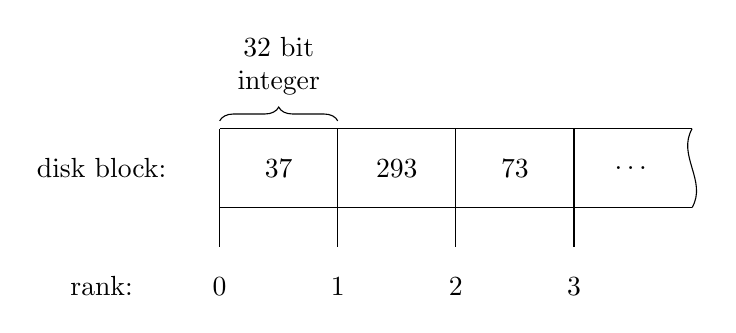
\begin{tikzpicture}[node distance={15mm}, main/.style = {draw, circle}]

    \draw (0,0) -- (6,0);
    \draw (0,1) -- (6,1);
    \draw (0,-0.5) -- (0,1);
    \draw (1.5,-0.5) -- (1.5,1);
    \draw (3,-0.5) -- (3,1);
    \draw (4.5,-0.5) -- (4.5,1);
    \draw[out=60, in=-120] (6,0) to (6,1);

    \node at (0.75, 0.5) {37};
    \node at (2.25, 0.5) {293};
    \node at (3.75, 0.5) {73};
    \node at (5.25, 0.5) {…};

    \node at (-1.5, 0.5) {disk block:};
    \node at (-1.5, -1) {rank:};
    \node at (0, -1) {0};
    \node at (1.5, -1) {1};
    \node at (3, -1) {2};
    \node at (4.5, -1) {3};

    \draw [decorate,decoration = {brace, amplitude=5pt}] (0,1.1) --  (1.5,1.1);
    \node[ align=center] at (0.75, 1.8) {32 bit  \\ integer};

\end{tikzpicture}
    \caption{Position File}
    \label{fig:position_file}
\end{figure}

\section{Reading Disk Arcs}

If one wants to get all upwards arcs of rank $i$ one need take  the upwards position file, retrieve the integer $j$ that is stored at index $i$, and then read the complete block $j$ in the upwards arc file. There
There one will get an array, contain the requested arcs but also some other. These arcs are likely to be request next. Therefore we want to keep them in memory. We implemented two buffer a \textit{circular buffer} and a \textit{least recently used buffer} LRU

\subsection{Circular Buffer}

For the circular buffer we simply used an array of disk arcs. If we reach the end of the buffer we restart overwriting the values from the array start. To get the all arcs of a rank one request that rank number. There is a position hash table which tells the start position of that rank inside the buffer. If it is missing, the containing disk block is read to the buffer. It 
continues to read sequentially until the request rank and the read arc doesn't belong together anymore. This buffer has the advantage that we can exactly determine the amount of arcs we buffering. Also as it is just a simple array, it will be easy for the operation system to cache it.
The disadvantage is that it is possible that we request arc sets very often as it is possible they get evicted just before request again.

\subsection{Least Recently Used Buffer}

Cache is a \textit{java.util.LinkedHashMap}. This class provides the possibility to evicted the entry that has been requested longest time ago. In our case it maps ranks to sets of disk arcs. We can only determine how many 
disk arc sets we have in memory and disk arc sets do not have always the same size. Higher rank vertex usually have bigger sets as they are of higher degree. The advantage is, it is very easy to implement and therefore very 
resilient to programming errors.

\section{The Search}

The search brings all things explained in this chapter together. 

%\begin{figure}
%    \centering
%    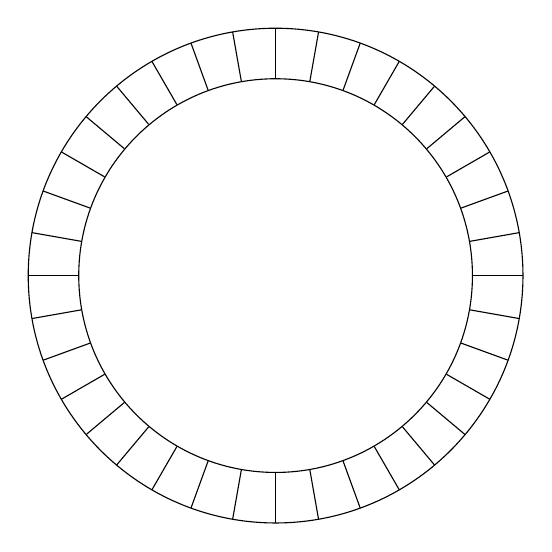
\begin{tikzpicture}[node distance={15mm}, main/.style = {draw, circle}]

    \draw (0,0) node[main, minimum size=5cm](z0) {} circle (pi);
    \draw (z0) -- (10:pi) node[midway,above]{};
    \draw (z0) -- (20:pi) node[midway,above]{};
    \draw (z0) -- (30:pi) node[midway,above]{};
    \draw (z0) -- (40:pi) node[midway,above]{};
    \draw (z0) -- (50:pi) node[midway,above]{};
    \draw (z0) -- (60:pi) node[midway,above]{};
    \draw (z0) -- (70:pi) node[midway,above]{};
    \draw (z0) -- (80:pi) node[midway,above]{};
    \draw (z0) -- (90:pi) node[midway,above]{};
    \draw (z0) -- (100:pi) node[midway,above]{};
    \draw (z0) -- (110:pi) node[midway,above]{};
    \draw (z0) -- (120:pi) node[midway,above]{};
    \draw (z0) -- (130:pi) node[midway,above]{};
    \draw (z0) -- (140:pi) node[midway,above]{};
    \draw (z0) -- (150:pi) node[midway,above]{};
    \draw (z0) -- (160:pi) node[midway,above]{};
    \draw (z0) -- (170:pi) node[midway,above]{};
    \draw (z0) -- (180:pi) node[midway,above]{};
    \draw (z0) -- (190:pi) node[midway,above]{};
    \draw (z0) -- (200:pi) node[midway,above]{};
    \draw (z0) -- (210:pi) node[midway,above]{};
    \draw (z0) -- (220:pi) node[midway,above]{};
    \draw (z0) -- (230:pi) node[midway,above]{};
    \draw (z0) -- (240:pi) node[midway,above]{};
    \draw (z0) -- (250:pi) node[midway,above]{};
    \draw (z0) -- (260:pi) node[midway,above]{};
    \draw (z0) -- (270:pi) node[midway,above]{};
    \draw (z0) -- (280:pi) node[midway,above]{};
    \draw (z0) -- (290:pi) node[midway,above]{};
    \draw (z0) -- (300:pi) node[midway,above]{};
    \draw (z0) -- (310:pi) node[midway,above]{};
    \draw (z0) -- (320:pi) node[midway,above]{};
    \draw (z0) -- (330:pi) node[midway,above]{};
    \draw (z0) -- (340:pi) node[midway,above]{};
    \draw (z0) -- (350:pi) node[midway,above]{};
    \draw (z0) -- (0:pi) node[midway,above]{};
    
\end{tikzpicture}
%    \caption{Circular Buffer}
%    \label{fig:circular_buffer}
%\end{figure}

\chapter{Important Algorithms}

\section{Updating a Priority Queue}

\section{Search Algorithm}

\newpage
\section{Triangles}

\begin{figure}
    \centering
    \begin{tikzpicture}[node distance={15mm}, main/.style = {draw, circle}]
    \node[rotate=90] at (-0.25,0) {rank};
    \draw [ -Stealth]  (0,-2) -- (0,2);
    \node[main] (x1) at (1, 0) {$x$}; 
    \node[main] (z1) [below right of=x1] {$z$};
    \node[main] (y1) [right of=z1, above of=x1] {$y$}; 
    \draw (x1) -- node[above left, sloped] {$a$} (y1) ;
    \draw (x1) -- node[below left, sloped, pos=0.8] {$b$} (z1);
    \draw (y1) -- node[below left, sloped] {$c$} (z1);
    \node[] at (2,-2) {lower triangle $\{x,y\}$};
    
    \node[main] (z2) at (6, 0) {$z$}; 
    \node[main] (x2) [below right of=z2] {$x$};
    \node[main] (y2) [right of=z2, above of=z2] {$y$}; 
    \draw (z2) -- node[above left, sloped] {$c$} (y2) ;
    \draw (z2) -- node[below left, sloped, pos=0.8] {$b$} (x2);
    \draw (y2) -- node[below left, sloped] {$a$} (x2);
    \node[] at (7,-2) {intermediate triangle $\{x,y\}$};
    
    \node[main] (y3) at (12, 0) {$y$}; 
    \node[main] (x3) [below right of=y3] {$x$};
    \node[main] (z3) [right of=y3, above of=y3] {$z$}; 
    \draw (y3) -- node[above left, sloped] {$c$} (z3);
    \draw (y3) -- node[below left, sloped, pos=0.8] {$a$} (x3);
    \draw (z3) -- node[below left, sloped] {$b$} (x3);
    \node[] at (13,-2) {upper Triangle $\{x,y\}$};
\end{tikzpicture}
    
    \caption{Triangle Enumeration}
    \label{fig:triangel enumeration}
\end{figure}

\begin{algorithm}
    \caption{Compute Triangles}
    \begin{algorithmic}[1]
    
    \Procedure{lowerTriangles}{$arc, neighbors$}
    \State $\text{triangles} \gets$ \{\}; 
    $\text{x} \gets$ min(arc.start, arc.end);
    $\text{y} \gets$ max(arc.start, arc.end);
    \ForAll{$z$ in $neighbors$}
        \If{$z < x < y$}
            \If{$\text{upwards}(arc)$}
                 $\text{triangles.add}(\text{Triangle}(arc, x.\text{getArcTo}(z), z.\text{getArcTo}(y)))$
            \Else  $\text{ triangles.add}(\text{Triangle}(arc, z.\text{getArcTo}(x), y.\text{getArcTo}(z)))$
            \EndIf
        \EndIf
    \EndFor
    \State \textbf{return} $\text{triangles}$
    \EndProcedure
    
    \Procedure{intermediateTriangles}{$arc, neighbors$}
    \State $\text{triangles} \gets$ \{\};
    $\text{x} \gets$ min(arc.start, arc.end);
    $\text{y} \gets$ max(arc.start, arc.end);
    \ForAll{$z$ in $neighbors$}
        \If{$x < z < y$}
            \If{$\text{upwards}(arc)$}
                 $\text{triangles.add}(\text{Triangle}(arc, z.\text{getArcTo}(x), z.\text{getArcTo}(y)))$
            \Else  $\text{ triangles.add}(\text{Triangle}(arc, x.\text{getArcTo}(z), y.\text{getArcTo}(z)))$
            \EndIf
        \EndIf
    \EndFor
    \State \textbf{return} $\text{triangles}$
    \EndProcedure
    
    \Procedure{upperTriangles}{$arc, neighbors$}
    \State $\text{triangles} \gets$ \{\};
    $\text{x} \gets$ min(arc.start, arc.end);
    $\text{y} \gets$ max(arc.start, arc.end);
    \ForAll{$z$ in $neighbors$}
        \If{$x < y < z$}
            \If{$\text{upwards}(arc)$}
                 $\text{triangles.add}(\text{Triangle}(arc, z.\text{getArcTo}(x), z.\text{getArcTo}(y)))$
            \Else  $\text{ triangles.add}(\text{Triangle}(arc, x.\text{getArcTo}(z), y.\text{getArcTo}(z)))$
            \EndIf
        \EndIf
    \EndFor
    \State \textbf{return} $\text{triangles}$
    \EndProcedure
    
    \end{algorithmic}
    \end{algorithm}
    

\bibliography{related.bib}
\addcontentsline{toc}{chapter}{Bibliography}


\end{document}
